\documentclass[12pt]{article}
\usepackage{a4wide}
\usepackage{color, amssymb}
\usepackage[margin=1in]{geometry}
\usepackage[document]{ragged2e}
\usepackage[table]{xcolor}
\usepackage{multirow}
\usepackage[braket, qm]{qcircuit}
\setlength{\arrayrulewidth}{0.5mm}
\setlength{\tabcolsep}{16pt}
\renewcommand{\arraystretch}{1.9}
\usepackage[english,greek]{babel}
\usepackage{braket}
\usepackage{mathtools}
\usepackage{ragged2e}
\renewcommand{\baselinestretch}{1.5}
\input{epsf}
\usepackage{float}
\usepackage{graphicx}
\usepackage{caption}
\usepackage{subcaption}
\usepackage{algorithm}
\usepackage[noend]{algpseudocode}

\begin{document}

\greektext

\noindent\rule{\textwidth}{2pt}
\begin{center}
{\bf ΚΒΑΝΤΙΚΗ ΤΕΧΝΟΛΟΓΙΑ}\\ 
{\bf 1o Σετ Ασκήσεων }\\
{\bf Καλαμαράκης Θεόδωρος:} 2018030022\\
\end{center}
\rule{\textwidth}{.5pt}
\noindent

\begin{center}

\end{center}
 
 

\justifying

\section*{{\bf Μέρος  $\bf 2^o$ }}

\rule{\textwidth}{.5pt}
%%%%%%%%%%%%%%%%%%%%%%%%%%%%%%%%%%%%%%%%%%%%%%%%%%%%%%%%%%%%%%%%%%%%%%%%%%%%%%%%%%%%%%%%%%%%%%%%%%%%%%%%%%%%%%%%%%%%%%%%%%%%%%%%%%%%%%%
\section*{{\bfΆσκηση 2}}
\subsubsection*{Απόδειξη σχέσης $(3.25)$}
Απο την σχέση $(3.24)$ έχουμε 
$$ \hat{H}'(t) = - \hbar\frac{\omega_0\hat{\sigma}_z}{2} +\frac{\hbar\gamma}{2}\left(B_0 \hat{\sigma}_z +e^{i\frac{\omega_0\hat{\sigma}_z}{2}t}B_1\cos(\omega\cdot t)\cdot\hat{\sigma}_x e^{-i\frac{\omega_0\hat{\sigma}_z}{2}t}\right) $$
Χρησιμοποιώντας οτι $\gamma B_0 = \omega_0$ η $(3.24)$ γίνεται :
\begin{align*}
    \hat{H}'(t) &= - \hbar\frac{\omega_0\hat{\sigma}_z}{2} +\hbar\frac{\omega_0\hat{\sigma}_z}{2}+\frac{\hbar\gamma}{2}\left( e^{i\frac{\omega_0\hat{\sigma}_z}{2}t}B_1\cos(\omega\cdot t)\cdot\hat{\sigma}_x e^{-i\frac{\omega_0\hat{\sigma}_z}{2}t}\right)=\\   
                &=\frac{\hbar\gamma}{2}\left( e^{i\frac{\omega_0\hat{\sigma}_z}{2}t}B_1\cos(\omega\cdot t)\cdot\hat{\sigma}_x e^{-i\frac{\omega_0\hat{\sigma}_z}{2}t}\right)
\end{align*}
Χρησιμοποιώντας οτι $2\cos(\omega \cdot t) = e^{i\omega t} + e^{-i\omega t}$ και οτι $\hat{\sigma}_x = \hat{\sigma}_+ + \hat{\sigma}_-$ (προκύπτει απο την $(3.21)$)
\begin{align*}
    \hat{H}'(t) &=\frac{\hbar\gamma}{2}\left( e^{i\frac{\omega_0\hat{\sigma}_z}{2}t}B_1\cos(\omega\cdot t)\cdot\hat{\sigma}_x e^{-i\frac{\omega_0\hat{\sigma}_z}{2}t}\right) =\\
                &=  \frac{\hbar\gamma}{2}\left( e^{i\frac{\omega_0\hat{\sigma}_z}{2}t}B_1(e^{i\omega t} + e^{-i\omega t})\cdot(\hat{\sigma}_+ + \hat{\sigma}_- )e^{-i\frac{\omega_0\hat{\sigma}_z}{2}t}\right) =\\
                &=  \frac{\hbar\gamma}{2}\left( e^{i\frac{\omega_0\hat{\sigma}_z}{2}t}B_1(e^{i\omega t}\hat{\sigma}_+ + e^{-i\omega t}\hat{\sigma}_+ + e^{i\omega t}\hat{\sigma}_- + e^{-i\omega t}\hat{\sigma}_- )e^{-i\frac{\omega_0\hat{\sigma}_z}{2}t}\right) =\\
                &=  \frac{\hbar\gamma}{2}B_1(e^{i\omega t}e^{i\frac{\omega_0\hat{\sigma}_z}{2}t}\hat{\sigma}_+e^{-i\frac{\omega_0\hat{\sigma}_z}{2}t} + e^{-i\omega t}e^{i\frac{\omega_0\hat{\sigma}_z}{2}t}\hat{\sigma}_+e^{-i\frac{\omega_0\hat{\sigma}_z}{2}t} +\\
                &+ e^{i\omega t}e^{i\frac{\omega_0\hat{\sigma}_z}{2}t}\hat{\sigma}_-e^{-i\frac{\omega_0\hat{\sigma}_z}{2}t} + e^{-i\omega t}e^{i\frac{\omega_0\hat{\sigma}_z}{2}t}\hat{\sigma}_- e^{-i\frac{\omega_0\hat{\sigma}_z}{2}t})=\\
                &\stackrel{(3.23)}{=} \frac{\hbar\gamma}{2}B_1(e^{i\omega t}e^{i\omega_0 t}\hat{\sigma}_+ + e^{-i\omega t}e^{i\omega_0 t}\hat{\sigma}_+ + e^{i\omega t}e^{i\omega_0 t}\hat{\sigma}_ + e^{-i\omega t}e^{i\omega_0 t}\hat{\sigma}_- )=\\
                & = \frac{\hbar\gamma}{2}B_1\left[\left( e^{i(\omega_0 - \omega )t}\hat{\sigma}_+ + e^{i(\omega - \omega_0 )t}\hat{\sigma}_-\right) + \left( e^{i(\omega_0 + \omega )t}\hat{\sigma}_+ + e^{-i(\omega + \omega_0 )t}\hat{\sigma}_-\right) \right]
            \end{align*}
\subsubsection*{Απόδειξη σχέσης $(3.36)$}
Αντικαθιστώντας την σχέση $(3.33)$ στην σχέση $(3.31)$ 
$$\left\{
\begin{array}{lr}
i\left[\frac{d}{dt}(Ae^{\lambda t}) \right] = -\frac{\delta}{2}Ae^{\lambda t} + \frac{\Omega}{2}Be^{\lambda t}\\
i\left[\frac{d}{dt}(Be^{\lambda t}) \right] = \frac{\Omega}{2}Ae^{\lambda t} + \frac{\delta}{2}Be^{\lambda t}\\

\end{array}
\right\} \Rightarrow 
\left\{
\begin{array}{lr}
i\left[A\lambda e^{\lambda t} \right] = -\frac{\delta}{2}Ae^{\lambda t} + \frac{\Omega}{2}Be^{\lambda t}\\
i\left[B\lambda e^{\lambda t} \right] = \frac{\Omega}{2}Ae^{\lambda t} + \frac{\delta}{2}Be^{\lambda t}\\

\end{array}
\right\}
$$
$$
\left\{
\begin{array}{lr}
i\lambda +\frac{\delta}{2} = \frac{\Omega}{2}\frac{B}{A}\\
i\lambda - \frac{\delta}{2}= \frac{\Omega}{2}\frac{A}{B} \\

\end{array}
\right\} (1)\xRightarrow{\textnormal{ πολλαπασιάζουμε κατά μέλη}} -\lambda^2 -i\lambda\frac{\delta}{2} +  i\lambda\frac{\delta}{2} -\frac{\delta^2}{4} = \frac{\Omega^2}{4} \Leftrightarrow
$$
$$\Leftrightarrow \lambda^2 = -\left(\frac{\Omega^2}{4} + \frac{\delta^2}{4}\right) \Leftrightarrow \lambda_1 = i\frac{\sqrt{\Omega^2 + \delta^2}}{2} = i\frac{\Omega'}{2} \textnormal{ και } \lambda_2 = -i\frac{\sqrt{\Omega^2 + \delta^2}}{2}=-i\frac{\Omega'}{2}$$
Επιστέφοντας στη σχέση $(1)$ για $\lambda = \lambda_1$ 
έχουμε 
\begin{align*}
    \frac{B_1}{A_1} = \frac{\delta - \Omega'}{\Omega} \tag{2}
\end{align*}
για $\lambda = \lambda_2$ 
έχουμε 
\begin{align*}
    \frac{B_2}{A_2} = \frac{\delta + \Omega'}{\Omega} \tag{3}
\end{align*}
Αρα 
$$
\left\{
\begin{array}{lr}
    \alpha(t) = A_1 e^{\frac{i\Omega't}{2}}+ A_2 e^{\frac{-i\Omega't}{2}} \\
    b(t) = B_1 e^{\frac{i\Omega't}{2}} +B_2 e^{\frac{-i\Omega't}{2}}  \\

\end{array}
\right\} \xLeftrightarrow[(2),\;(3)]{A_1=a_1,\;A_2=a_2}
\left\{
\begin{array}{lr}
    \alpha(t) = a_1 e^{\frac{i\Omega't}{2}}+ a_2 e^{\frac{-i\Omega't}{2}} \\
    b(t) = \frac{\delta - \Omega'}{\Omega}a_1 e^{\frac{i\Omega't}{2}} +\frac{\delta + \Omega'}{\Omega}a_2 e^{\frac{-i\Omega't}{2}}  \\

\end{array}
\right\}
$$
\subsubsection*{Απόδειξη σχέσης $(3.37)$}
Απο τις δύο σχέσεις της $(3.36)$ λαμβάνουμε οτι 
$$
\left\{
\begin{array}{lr}
    \alpha(0) = a_1 e^{0}+ a_2 e^{0} \\
    b(0) = \frac{\delta - \Omega'}{\Omega}a_1 e^{0} +\frac{\delta + \Omega'}{\Omega}a_2 e^{0}  \\

\end{array}
\right\} = 
\left\{
\begin{array}{lr}
    \alpha(0) = a_1 + a_2  \\
    b(0) = \frac{\delta - \Omega'}{\Omega}a_1  +\frac{\delta + \Omega'}{\Omega}a_2   \\

\end{array}
\right\} =
$$
\begin{align*}
=\left\{
    \begin{array}{lr}
        \alpha(0) = a_1 + a_2  \\
        b(0) = \frac{\delta }{\Omega}(a_1+a_2)  -\frac{\Omega'}{\Omega}(a_1-a_2)   \\
    \end{array}
    \right\} =
    \left\{
    \begin{array}{lr}
        \alpha(0) = a_1 + a_2  \\
        \frac{\delta }{\Omega'}a(0)-\frac{\Omega}{\Omega'}b(0) =   a_1-a_2   \\
    \end{array}
    \right\}  \tag{4}
\end{align*}
Χρησιμοποιώντας τώρα οτι $e^{\frac{i\Omega't}{2}} = \cos(\frac{\Omega't}{2}) + i\sin(\frac{\Omega't}{2}) $  και $e^{\frac{-i\Omega't}{2}} = \cos(\frac{\Omega't}{2}) - i\sin(\frac{\Omega't}{2}) $ 
ξαναγράφουμε την $(3.37)$ ως:
$$
\left\{
\begin{array}{lr}
    \alpha(t) = a_1 \left(\cos(\frac{\Omega't}{2}) + i\sin(\frac{\Omega't}{2})\right)+ a_2 \left(cos(\frac{\Omega't}{2}) - i\sin(\frac{\Omega't}{2})\right)\\
    b(t) = \frac{\delta - \Omega'}{\Omega}a_1 \left(\cos(\frac{\Omega't}{2}) + i\sin(\frac{\Omega't}{2})\right) +\frac{\delta + \Omega'}{\Omega}a_2 \left(cos(\frac{\Omega't}{2}) - i\sin(\frac{\Omega't}{2})\right)  \\
\end{array}
\right\} =
$$
$$
=\left\{
\begin{array}{lr}
    \alpha(t) =  \cos(\frac{\Omega't}{2})(a_1+a_2) + i\sin(\frac{\Omega't}{2})(a_1-a_2) \\
    b(t) = \cos(\frac{\Omega't}{2})(\frac{\delta - \Omega'}{\Omega}a_1+\frac{\delta + \Omega'}{\Omega}a_2) +i\sin(\frac{\Omega't}{2})(\frac{\delta - \Omega'}{\Omega}a_1-\frac{\delta + \Omega'}{\Omega}a_2)  \\
\end{array}
\right\} =
$$
$$
=\left\{
\begin{array}{lr}
    \alpha(t) =  \cos(\frac{\Omega't}{2})(a_1+a_2) + i\sin(\frac{\Omega't}{2})(a_1-a_2) \\
    b(t) = \cos(\frac{\Omega't}{2})\left(\frac{\delta }{\Omega}(a_1+a_2)-\frac{\Omega'}{\Omega}(a_1-a_2)\right) +i\sin(\frac{\Omega't}{2})\left(\frac{\delta }{\Omega}(a_1-a_2)-\frac{\Omega'}{\Omega}(a_1+a_2)\right) \\
\end{array}
\right\} \stackrel{(4)}{=}
$$
$$
=\left\{
\begin{array}{lr}
    \alpha(t) =  \cos(\frac{\Omega't}{2})a(0) + i(\frac{\delta a(0)- \Omega b(0)}{\Omega'})\sin(\frac{\Omega't}{2}) \\
    b(t) = \cos(\frac{\Omega't}{2})\left(\frac{\delta }{\Omega}a(0)-\frac{\delta }{\Omega}a(0)+b(0)\right) +i\sin(\frac{\Omega't}{2})\left(\frac{\delta^2 }{\Omega\Omega'}a(0)-\frac{\delta}{\Omega'}b(0) -\frac{\Omega'}{\Omega}a(0)\right) \\
\end{array}
\right\} =
$$
$$
=\left\{
\begin{array}{lr}
    \alpha(t) =  \cos(\frac{\Omega't}{2})a(0) + i(\frac{\delta a(0)- \Omega b(0)}{\Omega'})\sin(\frac{\Omega't}{2}) \\
    b(t) = \cos(\frac{\Omega't}{2})b(0) +i\sin(\frac{\Omega't}{2})\left(-\frac{\delta}{\Omega'}b(0) +\frac{\delta^2 }{\Omega\Omega'}a(0)-\frac{\Omega'}{\Omega}a(0)\right) \\
\end{array}
\right\} \stackrel{(*)}{=}
$$
$$
=\left\{
\begin{array}{lr}
    \alpha(t) =  \cos(\frac{\Omega't}{2})a(0) + i(\frac{\delta a(0)- \Omega b(0)}{\Omega'})\sin(\frac{\Omega't}{2}) \\
    b(t) = \cos(\frac{\Omega't}{2})b(0) -i(\frac{\Omega a(0)+ \delta b(0)}{\Omega'})\sin(\frac{\Omega't}{2}) \\
\end{array}
\right\} 
$$
Όπου στο σημείο $(*)$ χρησιμοποιήσαμε οτι 
$$\frac{\delta^2 }{\Omega\Omega'}a(0)-\frac{\Omega'}{\Omega}a(0) = \frac{\delta^2 }{\Omega\Omega'}a(0)-\frac{\Omega'^2}{\Omega\Omega'}a(0)= \frac{\delta^2 -\Omega'^2}{\Omega\Omega'}a(0) = -\frac{\Omega^2}{\Omega\Omega'}a(0)=-\frac{\Omega}{\Omega'}a(0)$$
\rule{\textwidth}{.5pt}
\section*{{\bfΆσκηση 3}}
\subsubsection*{\textlatin{\bf i)}}
Απο την εξίσωση του \textlatin{Schrodinger} έχουμε οτι :
$$i\hbar\frac{\partial}{\partial t}\ket{\psi(t)} = \hat{H}\ket{\psi(t)} \Rightarrow  \ket{\psi(t)} = e^{-\frac{i\hat{H}t}{\hbar}}\ket{\psi(0)} = e^{-\frac{i\hbar\omega \sigma_x t}{\hbar}}\ket{0} = e^{-i\omega \sigma_x t}\ket{0}
$$
O πίνακας $\sigma_x$ έχει ιδιοδιανύσαματα τα $\ket{+},\ket{-}$ και ιδιοτιμές $+1,-1$. Αρα μπορεί να γραφτεί ως 
$$ \sigma_x = \ket{+}\bra{+} - \ket{-}\bra{-}$$
Αρα
$$e^{-i\omega \sigma_x t} = e^{-i\omega (+1) t}\ket{+}\bra{+}+ e^{-i\omega (-1) t}\ket{-}\bra{-} = e^{-i\omega t}\ket{+}\bra{+}+ e^{i\omega t}\ket{-}\bra{-}\Rightarrow$$
\begin{align*}
    \ket{\psi(t)} &= e^{-i\omega \sigma_x t}\ket{0} = \left(e^{-i\omega t}\ket{+}\bra{+}+ e^{i\omega t}\ket{-}\bra{-}\right)\ket{0}=\\
    &=e^{-i\omega t}\ket{+}\left(\frac{\braket{0|0}+\braket{1|0}}{\sqrt{2}}\right) + e^{i\omega t}\ket{-}\left(\frac{\braket{0|0}-\braket{1|0}}{\sqrt{2}}\right)=\\
    &=\frac{1}{\sqrt{2}}\left(e^{-i\omega t}\ket{+}+e^{i\omega t}\ket{-}\right) = \frac{1}{{2}}\left(e^{-i\omega t}(\ket{0}+ \ket{1})+e^{i\omega t}(\ket{0}- \ket{1})\right)=\\
    &=\frac{1}{{2}}\left((e^{-i\omega t}+ e^{i\omega t})\ket{0}+(e^{-i\omega t}- e^{i\omega t})\ket{1}\right)=\cos(\omega t)\ket{0} -i\sin(\omega t)\ket{1}
\end{align*}
\subsubsection*{\textlatin{\bf ii)}}
Η ζητούμενη πιθανότητα είναι :
$$|\braket{\psi(0)|\psi(t)}|^2 = |\cos(\omega t)\braket{0|0} -i\sin(\omega t)\braket{0|1}|^2 = |\cos(\omega t)|^2$$
Η παραπάνω ποσότητα εκφράζει την πιθανότητα η κατάσταση $\psi$ να είναι $\ket{0}$  σε κάθε χρονική στιγμή, η γραφική της αναπαράσταση είναι η εξής: 

\begin{figure}[H]

    \centering
    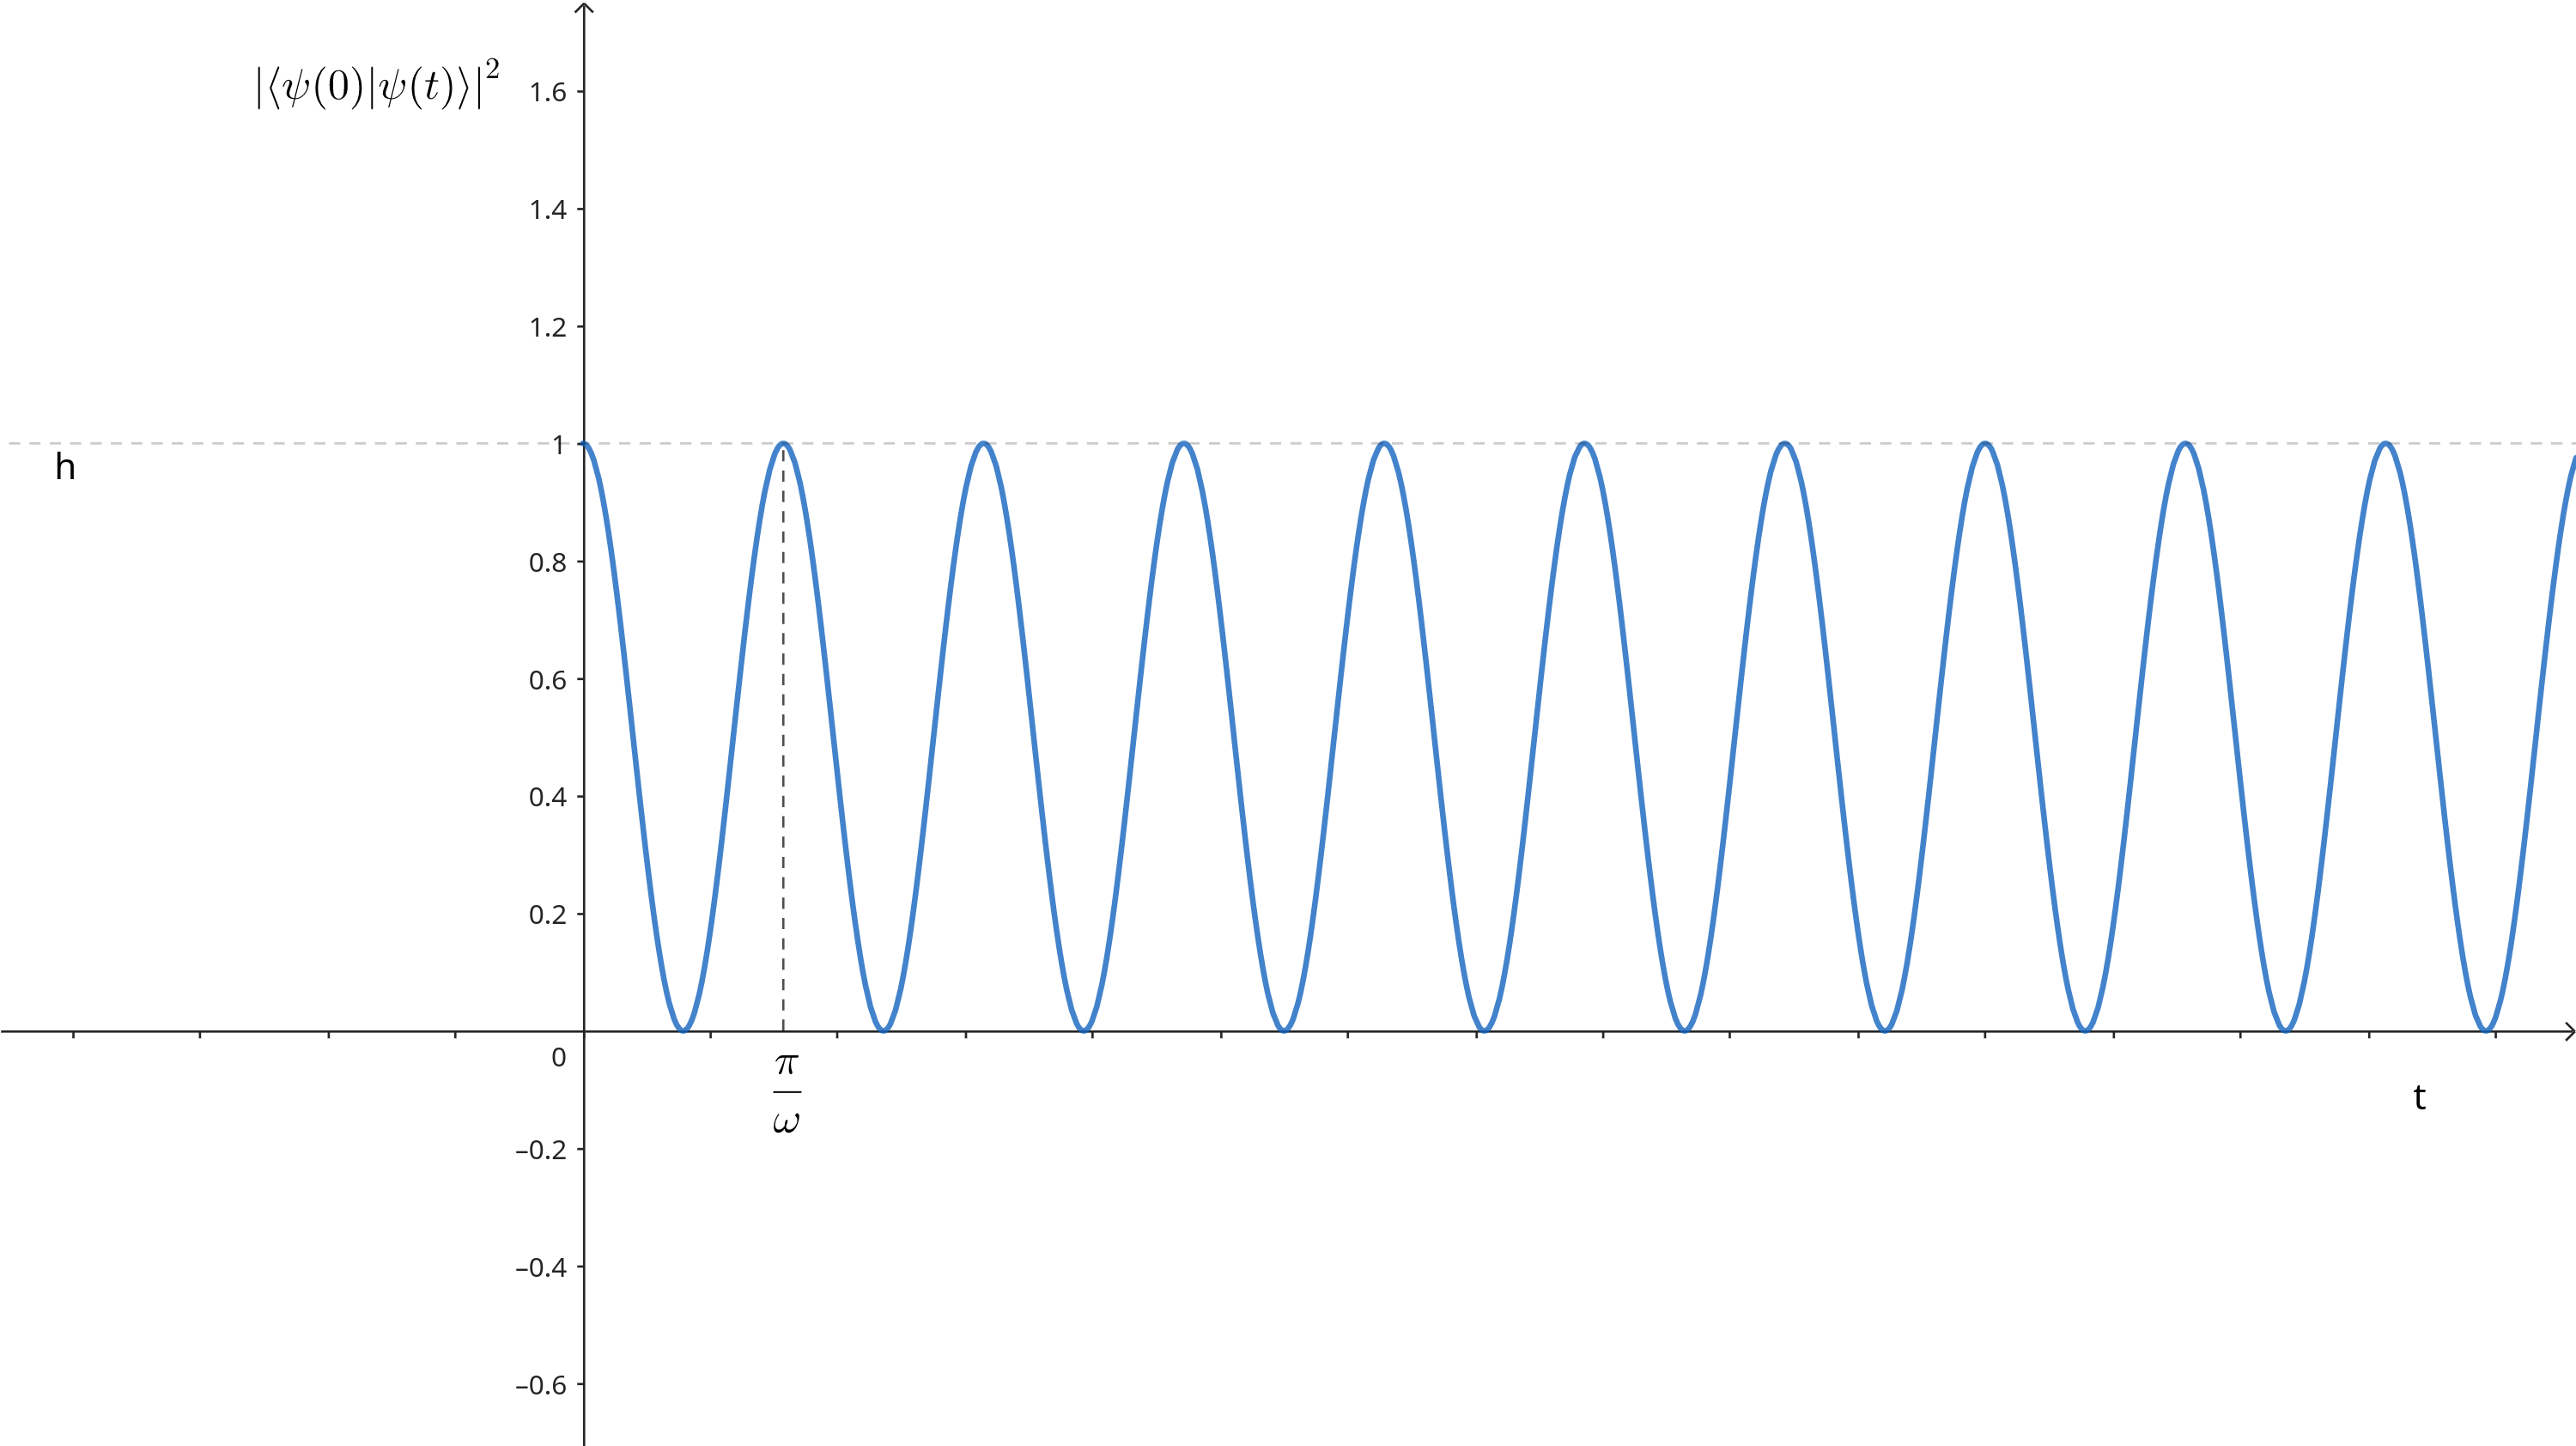
\includegraphics[scale = 0.4]{geogebra-export.png}\\ 
\end{figure}
\rule{\textwidth}{.5pt}
\section*{{\bfΆσκηση 4}}
\subsubsection*{\textlatin{\bf i)}}
Αρχικά υπολογίζουμε τον πινακα $H= J(X\otimes X+Y\otimes Y +Z\otimes Z)$


$$X\otimes X = X =\begin{bmatrix}
    0 & X \\ 
    X & 0
\end{bmatrix}= \begin{bmatrix}
    \;0 & 0& 0& 1 \;\\ 
    \;0 & 0& 1& 0\;\\
    \;0 & 1& 0& 0\;\\
    \;1 & 0& 0& 0\;
\end{bmatrix}$$

$$Y\otimes Y  =\begin{bmatrix}
    0 & -iY \\ 
    iY & 0
\end{bmatrix}= \begin{bmatrix}
    \;0 & 0& 0& -1 \;\\ 
    \;0 & 0& 1& 0\;\\
    \;0 & 1& 0& 0\;\\
    \;-1 & 0& 0& 0\;
\end{bmatrix}$$

$$Z\otimes Z  =\begin{bmatrix}
    Z & 0 \\ 
    0 & -Z
\end{bmatrix}= \begin{bmatrix}
    \;1 & 0& 0& 0 \;\\ 
    \;0 & -1& 0& 0\;\\
    \;0 & 0&-1& 0\;\\
    \;0 & 0& 0& 1\;
\end{bmatrix}$$
Αρα $$Η = J\begin{bmatrix}
    \;1 & 0& 0& 0 \;\\ 
    \;0 & -1& 2& 0\;\\
    \;0 & 2&-1& 0\;\\
    \;0 & 0& 0& 1\;
\end{bmatrix} $$


Έπειτα θετοντας $\ket{\psi(t)} = \begin{bsmallmatrix}
    a(t)\\ 
    b(t)\\
    c(t)\\
    d(t)\\
\end{bsmallmatrix}$  λύνουμε την έξισωση του \textlatin{Shrodinger}

$$i\hbar \frac{\partial}{\partial t} \ket{\psi(t)} = H\ket{\psi(t)}\Leftrightarrow i\hbar \begin{bmatrix}
    \frac{\partial}{\partial t}a(t)\\ 
    \frac{\partial}{\partial t}b(t)\\
    \frac{\partial}{\partial t}c(t)\\
    \frac{\partial}{\partial t}d(t)\\
\end{bmatrix}=H\begin{bmatrix}
    a(t)\\ 
    b(t)\\
    c(t)\\
    d(t)\\
\end{bmatrix}$$
και θα προκύψει το σύστημα τεσσάρων διαφορικών εξισώσεων 

$$\left\{
    \begin{array}{lr}
        i\hbar\frac{\partial}{\partial t}\alpha(t) =  J a(t)\\
        i\hbar\frac{\partial}{\partial t}b(t) =  -J b(t) +2Jc(t)\\
        i\hbar\frac{\partial}{\partial t}c(t) =  2J b(t) -Jc(t)\\
        i\hbar\frac{\partial}{\partial t}d(t) =  J d(t)\\
    \end{array}
    \right\} $$

    Αφου προσδιορίσουμε τα $a(t),b(t),c(t),d(t)$ μέσω του παραπάνω συστήματος, θα λύσουμε τις εξισώσεις
    $$\left\{
    \begin{array}{lr}
        a(\tau) =  a(0)\\
        b(\tau) =  c(0)\\
        c(\tau) =  b(0)\\
        d(\tau) =  d(0)\\
    \end{array}
    \right\} $$ προκειμένου να υπολογίσουμε τον χρόνο $\tau$
\subsubsection*{\textlatin{\bf ii)}}
Θελουμε να υπολογίσουμε το 
$$(I\otimes H )\sqrt{\textnormal{\textlatin{SWAP}}}(Z\otimes I)\sqrt{\textnormal{\textlatin{SWAP}}} (S\otimes S^\dag)(I\otimes H ) =$$
$$(I\otimes H )\sqrt{\textnormal{\textlatin{SWAP}}}(Z\otimes I)\sqrt{\textnormal{\textlatin{SWAP}}}  \begin{bmatrix}
    \;1 & 0& 0& 0 \;\\ 
    \;0 & i& 0& 0\;\\
    \;0 & 0&i& 0\;\\
    \;0 & 0& 0& 1\;
\end{bmatrix}\frac{1}{\sqrt{2}} \begin{bmatrix}
    \;1 & 1& 0& 0 \;\\ 
    \;1 &-1&0& 0\;\\
    \;0 & 0&1& 1\;\\
    \;0 & 0& 1& -1\;
\end{bmatrix} =$$
$$(I\otimes H )\sqrt{\textnormal{\textlatin{SWAP}}}(Z\otimes I) \begin{bmatrix}
    \;1 & 0& 0& 0 \;\\ 
    \;0 & \frac{1}{2}(1+i)& \frac{1}{2}(1+i)& 0\;\\
    \;0 & \frac{1}{2}(1-i)&\frac{1}{2}(1+i)& 0\;\\
    \;0 & 0& 0& 1\;
\end{bmatrix}\frac{1}{\sqrt{2}} \begin{bmatrix}
    \;1 & 1& 0& 0 \;\\ 
    \;i &-i&0& 0\;\\
    \;0 & 0&i& i\;\\
    \;0 & 0& i& -i\;
\end{bmatrix} =$$
$$(I\otimes H )\sqrt{\textnormal{\textlatin{SWAP}}} \begin{bmatrix}
    \;1 & 0& 0& 0 \;\\ 
    \;0 & 1&0& 0\;\\
    \;0 & 0&-1& 0\;\\
    \;0 & 0& 0& -1\;
\end{bmatrix}\frac{1}{\sqrt{2}} \begin{bmatrix}
    \;1 & 1& 0& 0 \;\\ 
    \;\frac{1}{2}(-1+i) & \frac{1}{2}(1-i)& \frac{1}{2}(-1+i)& \frac{1}{2}(-1+i)\;\\
    \;\frac{1}{2}(1+i) & \frac{1}{2}(-1-i)&\frac{1}{2}(-1+i)& \frac{1}{2}(-1+i)\;\\
    \;0 & 0& i& -i\;
\end{bmatrix} =$$
$$(I\otimes H ) \begin{bmatrix}
    \;1 & 0& 0& 0 \;\\ 
    \;0 & \frac{1}{2}(1+i)& \frac{1}{2}(1+i)& 0\;\\
    \;0 & \frac{1}{2}(1-i)&\frac{1}{2}(1+i)& 0\;\\
    \;0 & 0& 0& 1\;
\end{bmatrix}\frac{1}{\sqrt{2}} \begin{bmatrix}
    \;1 & 1& 0& 0 \;\\ 
    \;\frac{1}{2}(-1+i) & \frac{1}{2}(1-i)& \frac{1}{2}(-1+i)& \frac{1}{2}(-1+i)\;\\
    \;-\frac{1}{2}(1+i) & -\frac{1}{2}(-1-i)&-\frac{1}{2}(-1+i)& -\frac{1}{2}(-1+i)\;\\
    \;0 & 0& -i& i\;
\end{bmatrix} =...$$
%%%%%%%%%%%%%%%%%%%%%%%%%%%%%%%%%%%%%%%%%%%%%%%%%%%%%%%%%%%%%%%%%%%%%%%%%%%%%%%%%%%%%%%%%%%%%%%%%%%%%%%%%%%%%%%%%%%%%%%%%%%%%%%%%%%%%%%


\end{document}